\section{Progettazione concettuale}

\subsection{Analisi delle entità}

%Imbarcazione
\begin{center}
    \begin{tabularx}{\textwidth}{|l|l|l|X|}
        \hline
        \rowcolor{gray!30}
        \multicolumn{4}{|c|}{\textbf{Imbarcazione}}\\
        \hline
        Codice internazionale & CHAR(9) & Identifica univocamente un'imbarcazione nel mondo & Chiave\\
        \hline
        Nome & VARCHAR & \multicolumn{2}{l|}{Il nome dell'imbarcazione} \\
        \hline
        QtPostiLetto & INTEGER & \multicolumn{2}{l|}{La quantità di posti letto dell'imbarcazione} \\
        \hline
        Nome del capitano & VARCHAR & \multicolumn{2}{l|}{Il nome del capitano} \\
        \hline
        Bandiera & VARCHAR & \multicolumn{2}{l|}{Nome dello stato di cui batte bandiera l'imbarcazione} \\
        \hline
        Dimensioni &  & \multicolumn{2}{l|}{Attributo composto: Pescaggio, Larghezza, LOA} \\
        \hline
        Pescaggio & DECIMAL & \multicolumn{2}{l|}{La misura del punto più in profondità dell'imbarcazione} \\
        \hline
        Larghezza & DECIMAL & \multicolumn{2}{l|}{La misura della larghezza al baglio massimo dell'imbarcazione} \\
        \hline
        LOA & DECIMAL & \multicolumn{2}{l|}{La misura della lunghezza fuoritutto dell'imbarcazione} \\
        \hline
    \end{tabularx}
\end{center}

%Molo
\begin{center}
    \begin{tabularx}{\textwidth}{|l|l|l|X|}
        \hline
        \rowcolor{gray!30}
        \multicolumn{4}{|c|}{\textbf{Molo}}\\

        \hline
        Numero molo & INTEGER & Identifica univocamente un molo & Chiave\\
        \hline
        Stato di occupazione & BOOLEAN &\multicolumn{2}{l|}{ Lo stato di occupazione del molo}\\
        \hline
        Dimensioni &  & \multicolumn{2}{l|}{Attributo composto: Profondità minima, Larghezza, Lunghezza} \\
        \hline
        Profondità minima & DECIMAL & \multicolumn{2}{l|}{La profondità misurata alla più bassa marea sizigiale} \\
        \hline
        Larghezza & DECIMAL & \multicolumn{2}{l|}{La misura della larghezza del molo} \\
        \hline
        Lunghezza & DECIMAL & \multicolumn{2}{l|}{La misura della lunghezza del molo} \\
        \hline
    \end{tabularx}
\end{center}

%servizio
\begin{center}
    \begin{tabularx}{\textwidth}{|l|l|l|X|}
        \hline
        \rowcolor{gray!30}
        \multicolumn{4}{|c|}{\textbf{Servizio}}\\
        \hline
        Nome & VARCHAR & Il nome del servizio & Chiave \\
        \hline
    \end{tabularx}
\end{center}


%Addetto
\begin{center}
    \begin{tabularx}{\textwidth}{|l|l|l|X|}
        \hline
        \rowcolor{gray!30}
        \multicolumn{4}{|c|}{\textbf{Addetto}}\\
        \hline
        Servizio & VARCHAR & È il servizio in cui lavora & \multirow{2}{*}{Chiave}\\
        \hhline{---}
        DataInizioContratto & DATE & È la data in cui il contratto è iniziat& \\
        \hline
        DataFineContratto & DATE &\multicolumn{2}{l|}{ È la data in cui il contratto è finito o finirà.}\\
        \hline
    \end{tabularx}
\end{center}

%Cliente
\begin{center}
    \begin{tabularx}{\textwidth}{|l|l|X|}
        \hline
        \rowcolor{gray!30}
        \multicolumn{3}{|c|}{\textbf{Cliente}}\\
        \hline
        Cittadinanza & VARCHAR & Lo stato di cui il cliente è cittadino\\
        \hline
        Residenza & VARCHAR & La città in cui il cliente è residente \\
        \hline
    \end{tabularx}
\end{center}

%Cliente occasionale
\begin{center}
    \begin{tabularx}{\textwidth}{|l|l|X|}
        \hline
        \rowcolor{gray!30}
        \multicolumn{3}{|c|}{\textbf{Cliente occasionale}}\\
        \hline
        Quantità di soste & INTEGER & Il numero di soste che il cliente ha effettuato presso la struttura \\
        \hline
    \end{tabularx}
\end{center}

%Cliente abituale
\begin{center}
    \begin{tabularx}{\textwidth}{|l|l|X|}
        \hline
        \rowcolor{gray!30}
        \multicolumn{3}{|c|}{\textbf{Cliente abituale}}\\
        \hline
        Sconto personale & DECIMAL & Lo sconto percentuale applicato alle sue fatture \\
        \hline
    \end{tabularx}
\end{center}

%Persona
\begin{center}
    \begin{tabularx}{\textwidth}{|l|l|l|X|}
        \hline
        \rowcolor{gray!30}
        \multicolumn{4}{|c|}{\textbf{Persona}}\\
        \hline
        CF & CHAR(16) & Identifica univocamente una persona & Chiave \\
        \hline
        Nome & VARCHAR & \multicolumn{2}{l|}{Il nome della persona} \\
        \hline
        Cognome & VARCHAR & \multicolumn{2}{l|}{Il cognome della persona} \\
        \hline
        DataNascita & DATE & \multicolumn{2}{l|}{La data di nascita della persona} \\
        \hline
        Contatto & VARCHAR & \multicolumn{2}{l|}{I contatti della persona(multi-valore)} \\
        \hline
    \end{tabularx}
\end{center}

%Prenotazione
\begin{center}
    \begin{tabularx}{\textwidth}{|l|l|l|X|}
        \hline
        \rowcolor{gray!30}
        \multicolumn{4}{|c|}{\textbf{Prenotazione}}\\
        \hline
        CF & VARCHAR & Il codice fiscale del cliente prenotante & \multirow{3}{*}{Chiave}\\
        \hhline{---}
        Molo & INTEGER & Il molo prenotante &\\
        \hhline{---}
        Previsione arrivo & DATE & La data in cui si prevede il cliente arrivo &\\
        \hline
        Previsione partenza & DATE & \multicolumn{2}{l|}{La data in cui si prevede il cliente parta}\\
        \hline
        Sosta & SOSTA & \multicolumn{2}{l|}{La sosta in cui si è trasformata la presente prenotazione}\\
        \hline
    \end{tabularx}
\end{center}

%Sosta
\begin{center}
    \begin{tabularx}{\textwidth}{|l|l|l|X|}
        \hline
        \rowcolor{gray!30}
        \multicolumn{4}{|c|}{\textbf{Sosta}}\\
        \hline
        Imbarcazione & VARCHAR & Il codice internazionale dell'imbarcazione & \multirow{3}{*}{Chiave}\\
        \hhline{---}
        Molo & INTEGER & Il molo della sosta &\\
        \hhline{---}
        Data arrivo & TIMESTAMP & Data in cui l'imbarcazione ha ormeggiato & \\
        \hline
        Data partenza & TIMESTAMP & \multicolumn{2}{l|}{Data in cui l'imbarcazione ha sciolto gli ormeggi} \\
        \hline
    \end{tabularx}
\end{center}

%Allacciamento
\begin{center}
    \begin{tabularx}{\textwidth}{|l|l|l|X|}
        \hline
        \rowcolor{gray!30}
        \multicolumn{4}{|c|}{\textbf{Allacciamento}}\\
        \hline
        Nome & VARCHAR & Il nome che identifica la tipologia di allacciamento &Chiave\\
        \hline
        Prezzo unitario & DECIMAL & \multicolumn{2}{l|}{Il prezzo unitario dell'allacciamento}\\
        \hline
        Unità di misura & VARCHAR & \multicolumn{2}{l|}{L'unità di misura utilizzata per conteggiarne il consumo}\\
        \hline
    \end{tabularx}
\end{center}

%Periodo di apertura
\begin{center}
    \begin{tabularx}{\textwidth}{|l|l|l|X|}
        \hline
        \rowcolor{gray!30}
        \multicolumn{4}{|c|}{\textbf{Periodo di apertura}}\\
        \hline
        Giorno di apertura & CHAR(3) & Giorno a cui si riferisce l'orario di apertura &\multirow{3}{*}{Chiave}\\
        \hhline{---}
        Orario di apertura & TIME & Orario a cui il servizio apre nel giorno & \\
        \hhline{---}
        Orario di chiusura & TIME & Orario a cui il servizio cudehi nel giorno & \\
        \hline
    \end{tabularx}
\end{center}

%Consumo
\begin{center}
    \begin{tabularx}{\textwidth}{|l|l|l|X|}
        \hline
        \rowcolor{gray!30}
        \multicolumn{4}{|c|}{\textbf{Consumo}}\\

        \hline
        Cliente & VARCHAR & Cliente consumante & \multirow{3}{*}{Chiave} \\
        \hhline{---}
        Allacciamento & VARCHAR & il tipo di allacciamento consumato &\\
        \hhline{---}
        Data inizio lettura & TIMESTAMP & Momento dell'inizio del conteggio & \\
        \hline
        Data fine lettura & TIMESTAMP & \multicolumn{2}{l|}{Momento della fine del conteggio}\\
        \hline
        Quantità consumata & DECIMAL & \multicolumn{2}{l|}{La quantità consumata nel periodo} \\
        \hline
    \end{tabularx}
\end{center}

%Fattura
\begin{center}
    \begin{tabularx}{\textwidth}{|l|l|l|X|}
        \hline
        \rowcolor{gray!30}
        \multicolumn{4}{|c|}{\textbf{Fattura}}\\
        \hline

        \hline
        Cliente & VARCHAR & Cliente ricevente & \multirow{2}{*}{Chiave} \\
        \hhline{---}
        Data scadenza & DATE & Identifica la scadenza della fattura & \\
        \hline
        Pagato & TIMESTAMP & \multicolumn{2}{l|}{Identifica quando è stata pagata e lo stato del pagamento della fattura} \\
        \hline
    \end{tabularx}
\end{center}


\subsection{Generalizzazioni}

\begin{itemize}
    \item Persona è generalizzazione parziale esclusiva di Addetto;
    \item Persona è generalizzazione parziale esclusiva di Cliente;
    \item Cliente è generalizzazione totale esclusiva di cliente abituale e cliente occasionale;
\end{itemize}

\subsection{Analisi delle relazioni e delle cardinalità}

\begin{itemize}
    
    \item Molo - Allacciamento: \textbf{Fornitura}
    \begin{itemize}
        \item Un Molo possiede più allacciamenti o nessuno (0,N);
        \item Un allacciamento può essere posseduto da più moli o da nessuno(0,N);
    \end{itemize}

    \item Consumo - Allacciamento: \textbf{Utilizzo}
    \begin{itemize}
        \item Un consumo utilizza uno e un solo allacciamento(1,1);
        \item Un allacciamento può essere utilizzato da 0 a molti consumi(0,N);
    \end{itemize}

    \item Consumo - Fattura: \textbf{Riga fattura consumo}
    \begin{itemize}
        \item Un consumo è riga di una o nessuna fattura(0,1);
        \item Una fattura ha da 0 a molte righe relative ai consumi(0,N);
    \end{itemize}

    \item Sosta - Fattura: \textbf{Riga fattura sosta}
    \begin{itemize}
        \item Una sosta è riga di una o nessuna fattura(0,1);
        \item Una fattura ha da 0 a molte righe relative alle soste (0,N);
    \end{itemize}

    \item Fattura - Cliente: \textbf{Destinatario fattura}
    \begin{itemize}
        \item Una fattura è destinata ad uno e un solo cliente(0,1);
        \item Un cliente può avere da 0 a molte fatture destinategli(0,N);
    \end{itemize}

    \item Addetto - Servizio: \textbf{Gestione}
    \begin{itemize}
        \item Un addetto gestisce uno e un solo servizio (1,1);
        \item Un servizio è gestito da un addetto o da nessuno (0,1);
    \end{itemize}

    \item Servizio - Periodo apertura: \textbf{Apertura}
    \begin{itemize}
        \item Un servizio ha da uno a molte aperture(1,N);
        \item Periodo di apetura definisce aperte da uno a molti servizi (1,N);
    \end{itemize}

    \item Consumo - Cliente: \textbf{Consumazione}
    \begin{itemize}
        \item Un Cliente effettua da 0 a molte consumazioni di consumazione(0,N);
        \item Un consumo è consumazione di uno e un solo cliente (1,1);
    \end{itemize}

    \item Prenotazione - Molo: \textbf{Riserve}
    \begin{itemize}
        \item Una prenotazione Riserva uno e un solo molo (1,1);
        \item Un molo può essere riservato da più prenotazioni o da nessuna (0,N);
    \end{itemize}

    \item Cliente - Imbarcazione: \textbf{Proprietà}
    \begin{itemize}
        \item Un cliente può possedere più imbarcazioni(Almeno una) (1,N);
        \item Un imbarcazione è posseduta da una e una sola una persona oppure da nessuno\footnote{Barca abbandonata}(0,1);
    \end{itemize}
    
    \item Cliente - Prenotazione: \textbf{Prenotazioni effettuate}
    \begin{itemize}
        \item Un cliente può aver effettuato da 0 a molte prenotazioni(0,N);
        \item Una prenotazione può essere stata effettuata al massimo da un cliente (1,1);
    \end{itemize}

    \item Molo - Sosta: \textbf{M\_S}
    \begin{itemize}
        \item Un molo può accogliere da 0 a molte soste(0,N);
        \item Una sosta è relativa a uno e un solo molo(1,1);
    \end{itemize}

    \item Sosta - Imbarcazione: \textbf{S\_I}
    \begin{itemize}
        \item Una sosta è relativa ad una e una sola imbarcazione(1,1);
        \item Un imbarcazione può sostare da 0 a molte volte (0,N);
    \end{itemize}

    \item Prenotazione - Sosta: \textbf{Arrivato}
    \begin{itemize}
        \item Una prenotazione Arriva in 0 o 1 molo(0,1);
        \item Un sosta ha in arrivo da 0 a una prenotazione (0,N);
    \end{itemize}
    
\end{itemize}

\subsection{Schema ER concettuale}
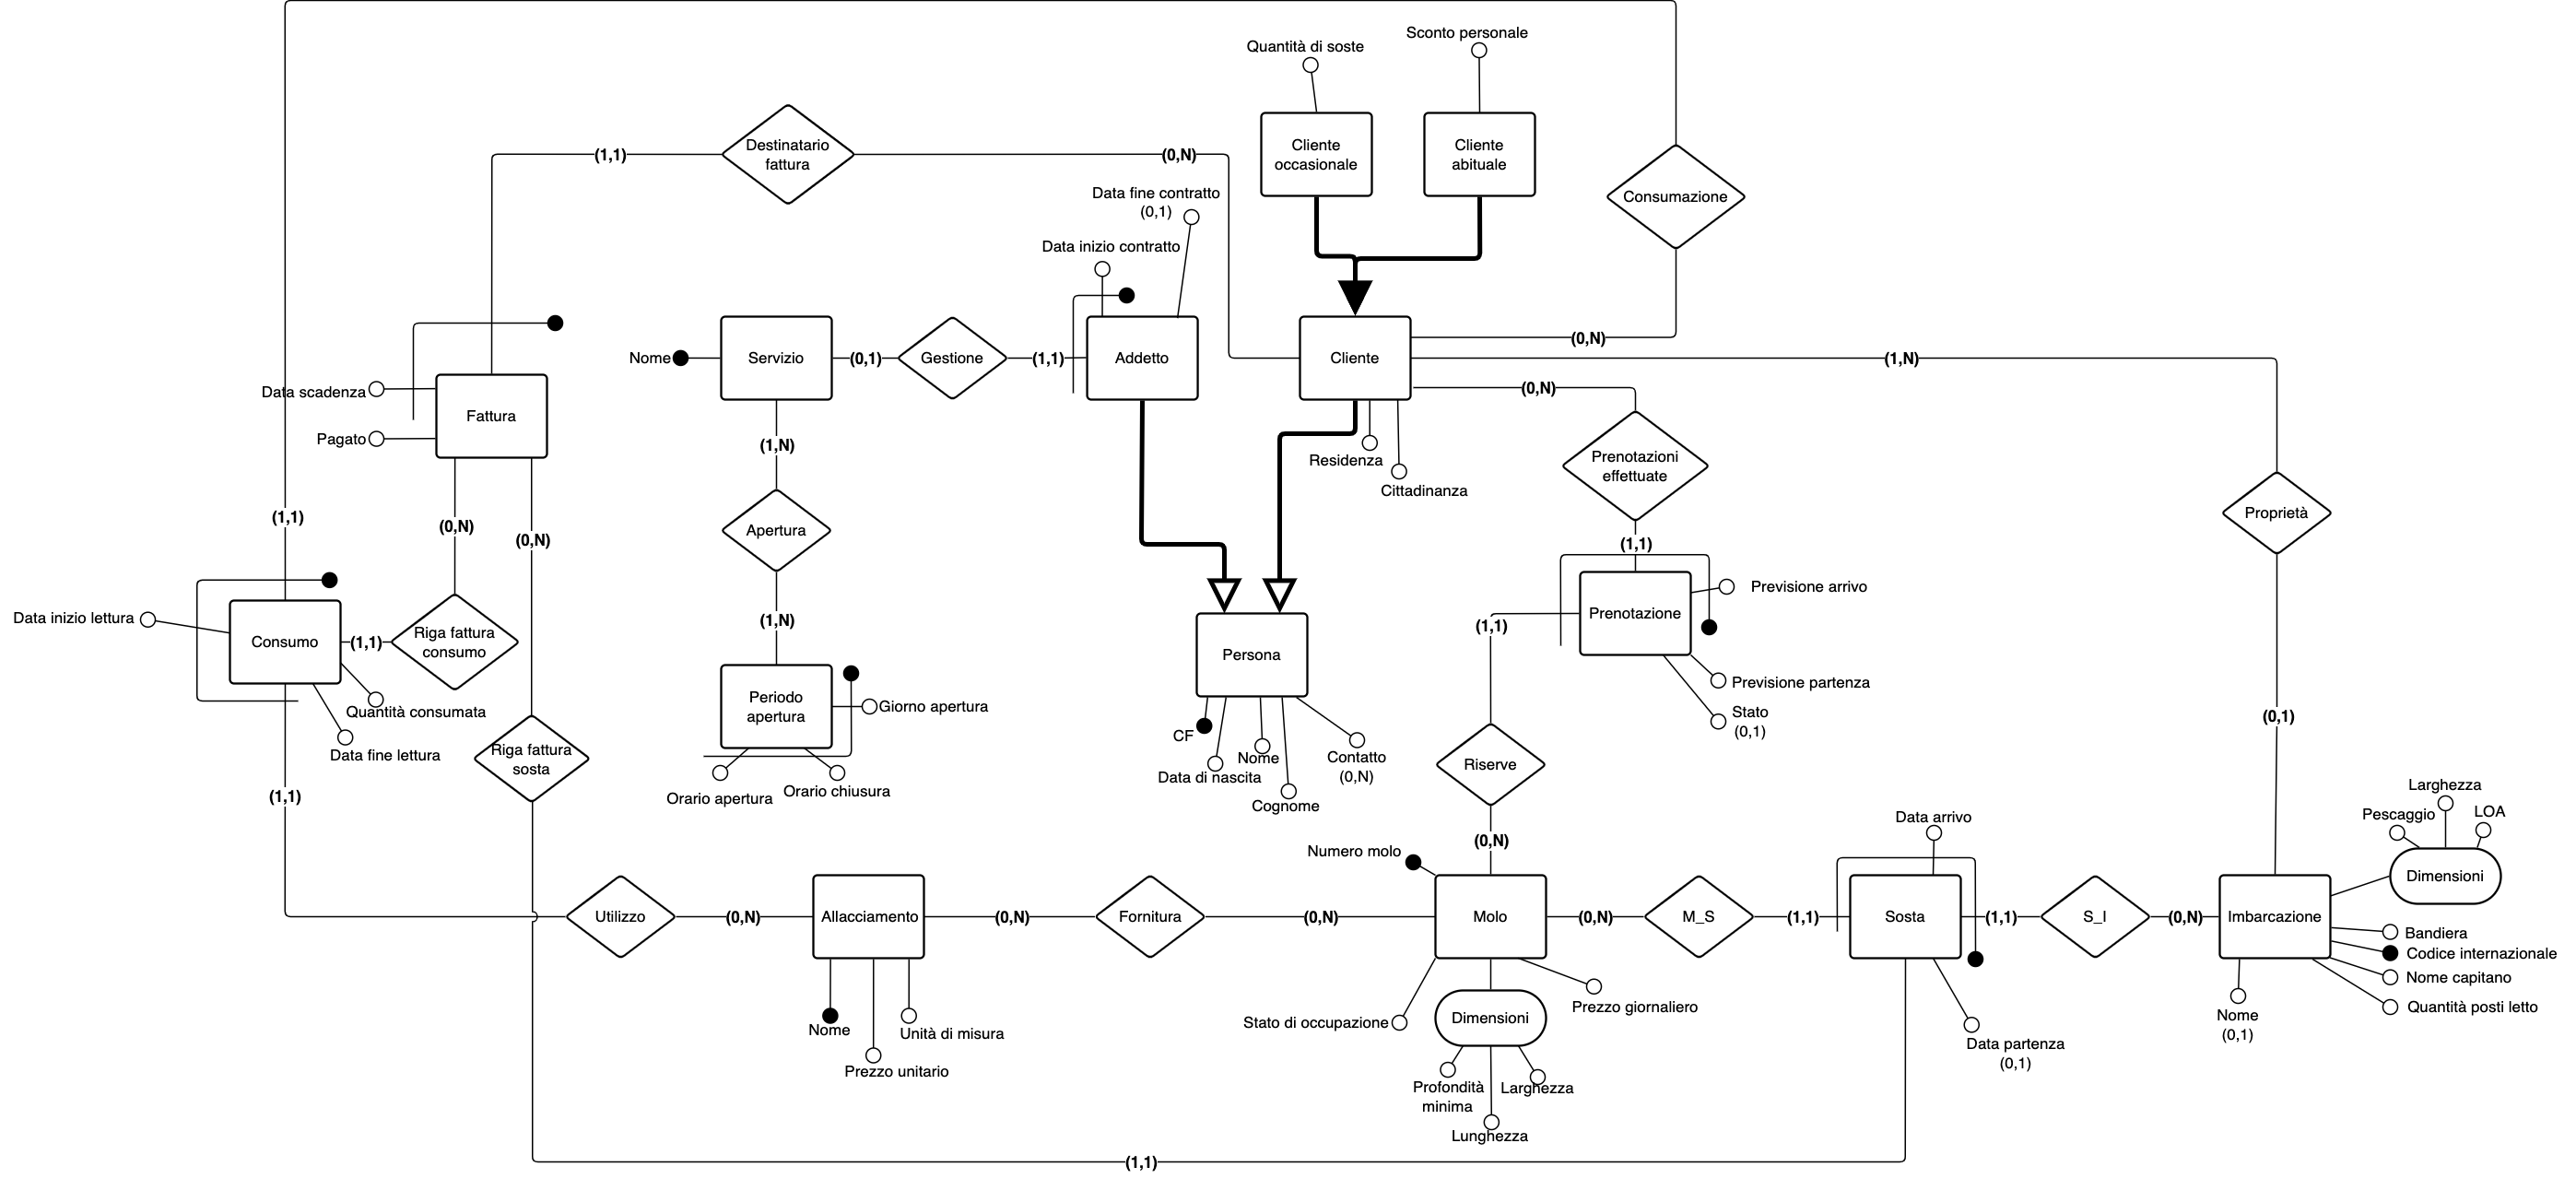
\includegraphics[width=\textwidth]{img/erconcettuale.png}

\subsubsection{Vincoli non rappresentabili nello schema Relazionale}

\begin{center}
    \begin{tabularx}{\textwidth}{|p{30mm}|X|}
        \hline
        \rowcolor{gray!30}
        \textbf{Entità / Relazione} & \textbf{Vincolo}\\
        \hline
        Molo & Lo stato di occupazione deve essere coerente con la sosta\\
        \hline

        Periodo di apertura & orario di chiusura deve essere postumo all'orario di apertura \\
        \hline

        Fattura & deve essere presente almeno una linea di consumo o una linea di sosta\\
        \hline

        Prenotazione & La previsione della partenza deve essere postuma alla previsione dell'arrivo\\
        \hline

        Prenotazione & Un molo non può essere prenotato nello stesso momento da due persone differenti e non può essere prenotato se c'è già una barca in sosta\\
        \hline

        Sosta & La data di partenza deve essere postuma alla data di arrivo\\

        \hline
        Sosta & Un molo non può essere utilizzato se è già occupato o è prenotato e un'imbarcazione non può occupare due moli contemporaneamente\\

        \hline
        Fattura& La data di pagamento di una fattura può essere solo postuma alla sua emissione\\

        \hline

        Consumo& L'inizio della lettura di un consumo è chiaramente precedente alla fine della stessa lettura\\
        \hline
    \end{tabularx}
\end{center}
